%*********************************************************************
\subsection{Simulation Experiment}\label{sub:bc_simulation_experiment}
%*********************************************************************

% Introductory paragraph

% The statistical calibration framework revisited

% Observation Layout

% Modeling the simulator output

% Modeling the discrepancy

% Likelihood Formulation

% Full Probability Model
% Different Model
% 1. TC, DP, and CO only
% 2. All Output, Discrepancy
% 3. All Output, No Discrepancy
% 4. 

Table~\ref{tab:ch5_calibration_schemes} summarizes the different calibration schemes considered in this study.
\begin{table*}[!htbp]\centering
\ra{0.9}
\begin{adjustwidth*}{}{-3cm}
\caption{Bayesian calibration schemes conducted for the \gls[hyper=false]{trace} reflood model parameters against data from \gls[hyper=false]{feba} test No. $216$.}
\label{tab:ch5_calibration_schemes}
\begin{tabular}{@{}clccccrc@{}}\toprule
\multirow{2}{*}{No.} & \multirow{2}{*}{\shortstack[c]{Calibration Scheme}} 	& \multirow{2}{*}{\shortstack[c]{Model Bias\\Term}}	& \multicolumn{3}{c}{Types of Output} & \phantom{a} & \multirow{2}{*}{\shortstack[c]{Reflood Model\\Parameters \footnotesize{(total number)}}} \\
																															  \cmidrule{4-6}
    &                                 					& 						& $TC$				& $DP$     		& $CO$   				&&	\\ \midrule
1   & \texttt{w/ Bias}	  											& \Checkmark  & \Checkmark  & \Checkmark  & \Checkmark  	&& All \footnotesize{($8$)}          				\\
2   & \texttt{w/ Bias, TC}     									& \Checkmark  & \Checkmark	&							&          			&& All \footnotesize{($8$)}           			\\
3   & \texttt{w/ Bias, DP}     									& \Checkmark 	&         		& \Checkmark	&								&& All \footnotesize{($8$)} 								\\
4   & \texttt{w/ Bias, CO}       								& \Checkmark 	& 						& 						& \Checkmark		&& All \footnotesize{($8$)}           			\\
5   & \texttt{w/o Bias}               					&          		& \Checkmark  & \Checkmark  & \Checkmark		&& All \footnotesize{($8$)}	          			\\
6   & \texttt{w/ Bias, no dffbVIHT}             & \Checkmark  & \Checkmark  & \Checkmark  & \Checkmark		&& Excluding \texttt{dffbVIHT} \footnotesize{(7)}\\
\bottomrule
\end{tabular}
\end{adjustwidth*}
\end{table*}

% Analyzing convergence
\clearpage
\begin{sidewaysfigure}
	\centering
	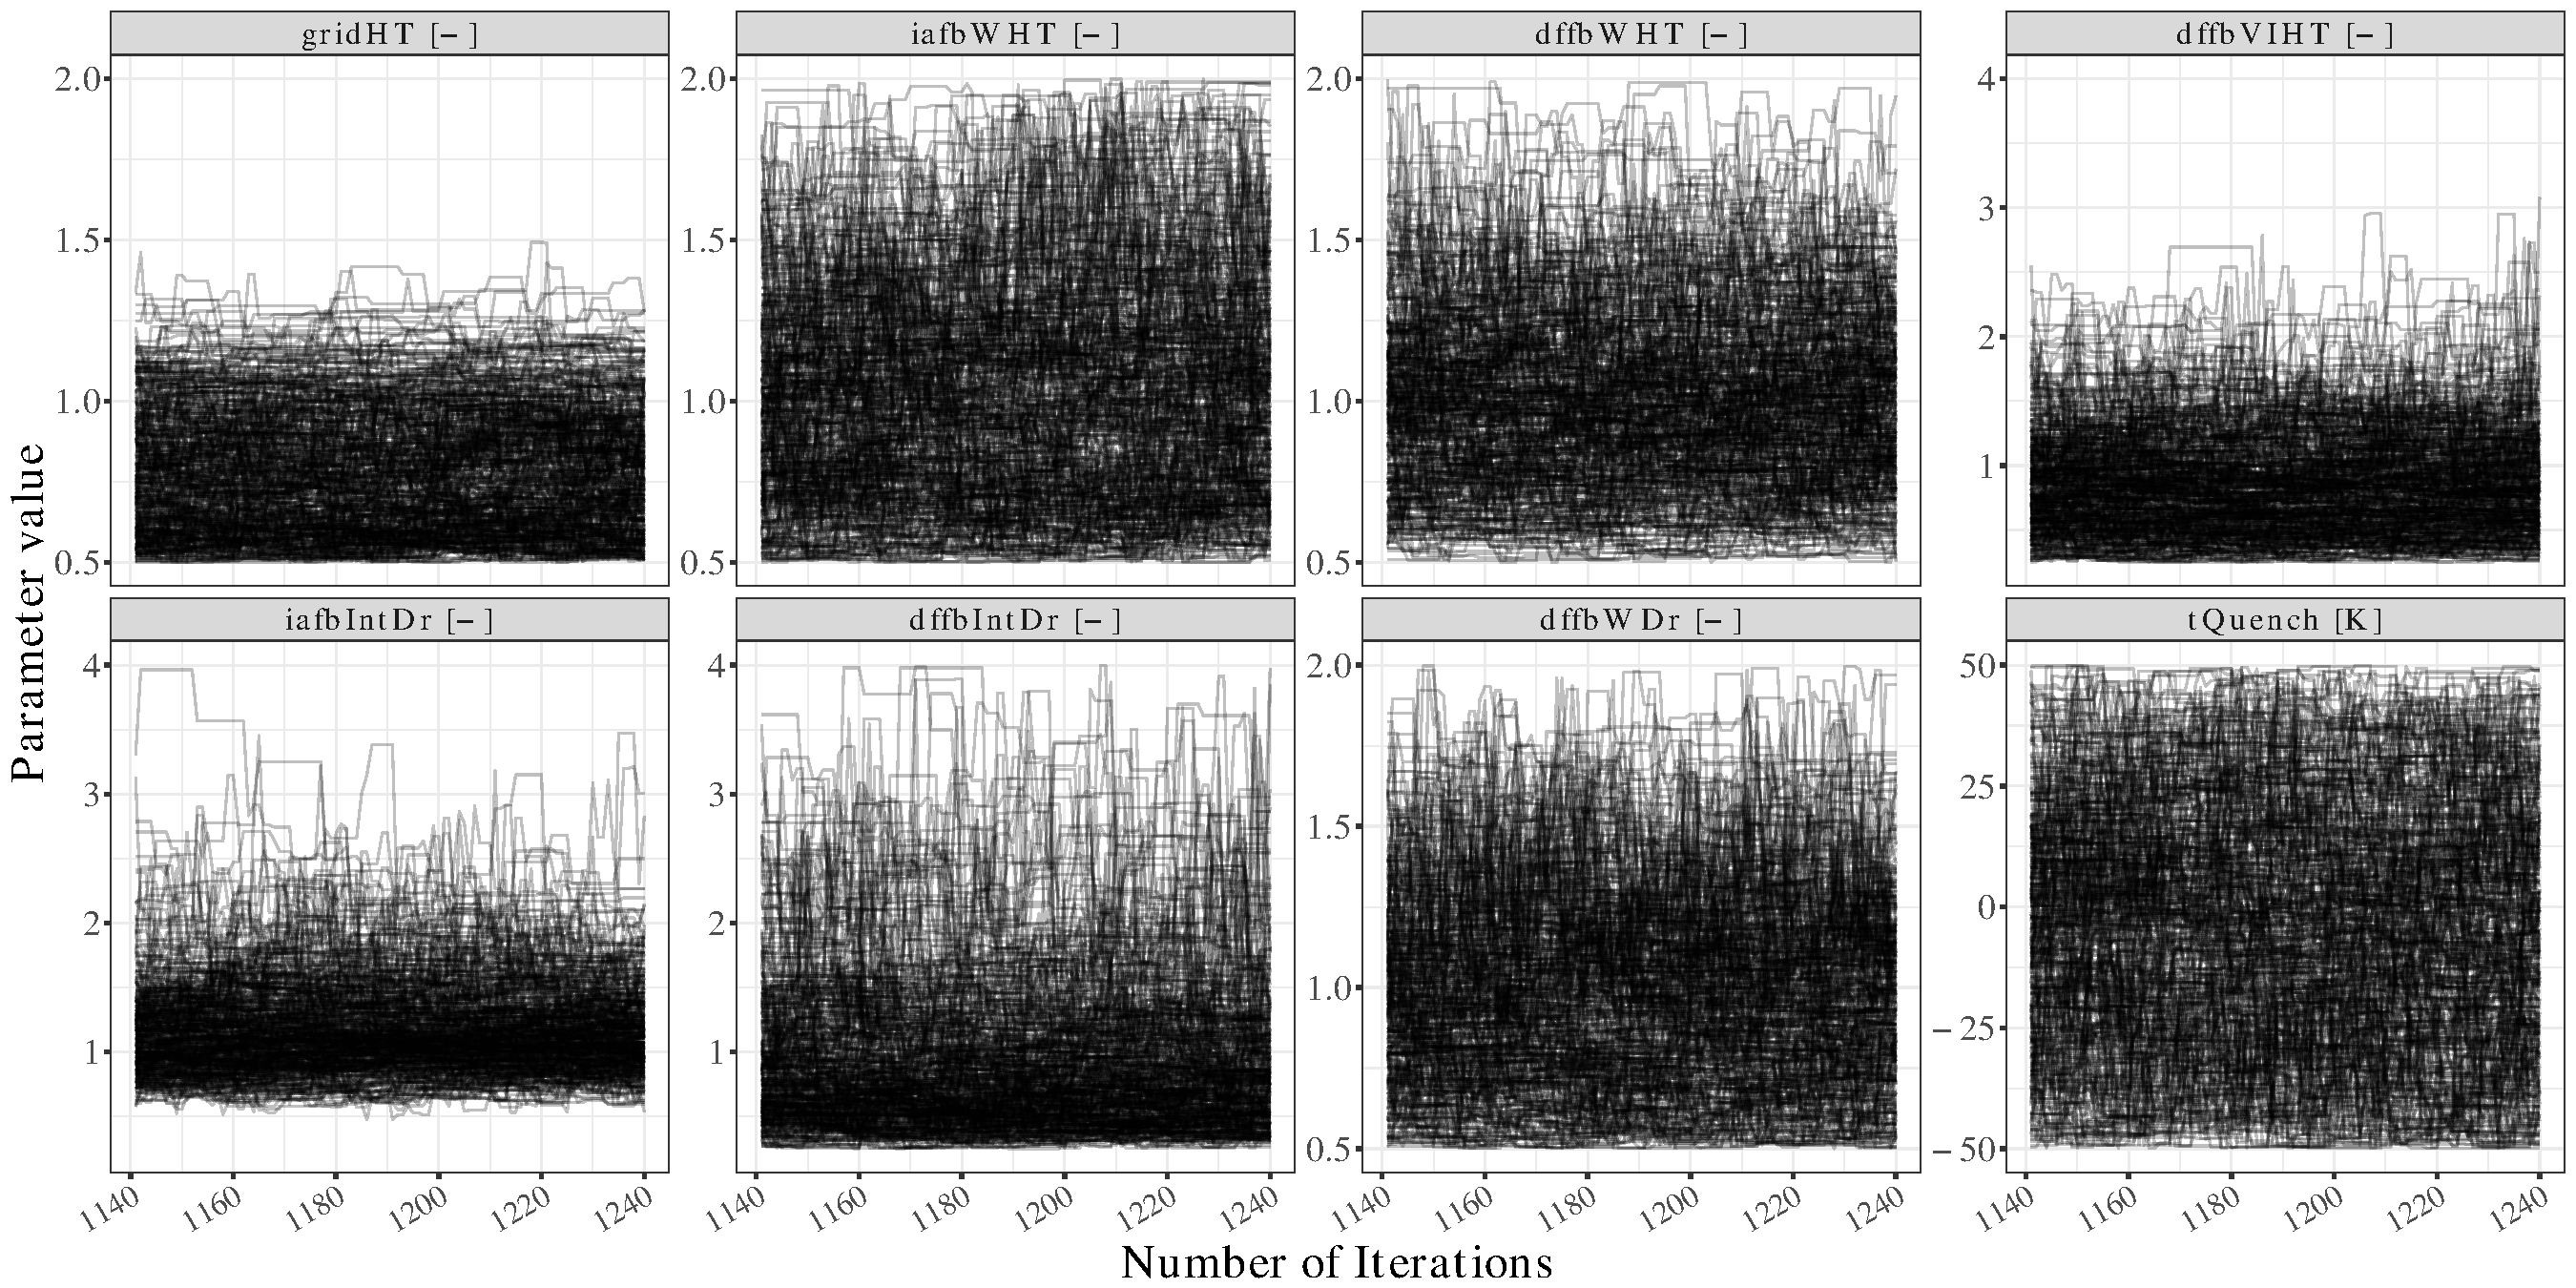
\includegraphics[width=0.90\textwidth]{../figures/chapter5/figures/plotEnsTraceDiscAllCentered}
		\captionof{figure}[Ensemble trace plots for each model parameter of calibration with model bias term.]{Ensemble trace plots for each model parameter of calibration with model bias term. Shown here is for the last $100$ iterations (out of $1'240$ post-burn-in iterations) and for $400$ walkers (out of $1'000$ walkers).}
	\label{fig:ch5_plot_ens_trace_all_disc_centered}
\end{sidewaysfigure}
\clearpage